\chapter{Propuesta}\label{cap:propuesta}

Este capítulo presenta el prototipo desarrollado en la Fase~3 (Sección~\ref{sec:fase3-caso}) recorriéndolo pantalla por pantalla. Para cada pantalla se describe qué hace, qué brecha del diagnóstico del SAE real aborda (Sección~\ref{sec:res-diagnostico}) y qué principio de diseño aplica, sea de la revisión de literatura (Sección~\ref{sec:que-funciona}) o de los marcos de diseño de interacción humano-IA (Sección~\ref{sec:fase3-marcos}). El capítulo describe lo que se construyó; si esas decisiones mejoran la comprensión, la confianza y la percepción de justicia de las familias es lo que responderá el estudio comparativo (Sección~\ref{sec:estudio-comparativo}), cuyos resultados aún no existen.

Las capturas se tomaron del prototipo en funcionamiento, a 390~píxeles de ancho ---el tamaño de un teléfono, que es el acceso principal del arquetipo Daniela González---, recorriendo el caso de la familia Muñoz González con la lista y el orden fijos del estudio comparativo. Todos los establecimientos, personas y cifras que aparecen en ellas son ficticios.

\section{Visión general}\label{sec:prop-general}

El prototipo es una aplicación web que reproduce los dos componentes del SAE evaluados en el diagnóstico: el sitio informativo y la plataforma de postulación. Se organiza en torno a tres momentos de la experiencia de una familia:

\begin{enumerate}
    \item \textbf{Informarse antes de postular}: buscar establecimientos, revisar su ficha, entender cómo funciona el algoritmo de asignación y conocer las etapas y fechas del proceso (Sección~\ref{sec:prop-informarse}).
    \item \textbf{Postular}: un flujo de tres pasos ---identificarse, armar y ordenar la lista de establecimientos, y revisar y enviar--- con los mismos datos y declaraciones que exige el SAE real (Sección~\ref{sec:prop-postular}).
    \item \textbf{Conocer el resultado}: ver el establecimiento asignado y por qué (Sección~\ref{sec:prop-resultado}).
\end{enumerate}

Sobre esas pantallas se aplican de manera transversal los principios de la interfaz: español de Chile con tuteo, lenguaje claro de nivel sexto básico, diseño pensado primero para el teléfono, un tamaño de letra base aumentado con una opción ``Grande'' visible en cada página, y texto de alto contraste (Sección~\ref{sec:accesibilidad}). Además, el mismo prototipo puede funcionar en una \textbf{condición de control} que oculta toda la capa de explicación del algoritmo, requerida por el estudio comparativo (Sección~\ref{sec:prop-control}).

\section{Informarse antes de postular}\label{sec:prop-informarse}

\textbf{Inicio y ficha de establecimiento.} La página de inicio (Figura~\ref{fig:prop-inicio}, izquierda) muestra en qué etapa del proceso se está y hasta cuándo se puede postular, calculado a partir del calendario oficial, y ofrece un recorrido guiado para quien entra por primera vez. Debajo, un buscador por nombre o comuna permite ordenar los establecimientos, entre otros criterios, por demanda o por vacantes. Aborda la brecha de \emph{búsqueda y encontrabilidad} del diagnóstico. La ficha de cada establecimiento reúne en una sola página su identidad institucional, sus vacantes y postulantes del año anterior, y una estimación de la probabilidad de obtener un cupo sin ninguna prioridad, expresada como ``26 de cada 100 postulantes'' junto a una matriz de cien íconos (Figura~\ref{fig:prop-inicio}, derecha). Ese formato de frecuencia, en lugar de un porcentaje aislado, responde a la evidencia sobre comunicación de riesgo para audiencias con numeracidad básica-intermedia recogida en los marcos de diseño, y combina gráfico y cifra según el principio de presentación multidimensional.

\begin{figure}[htbp]
\centering
\begin{minipage}[t]{0.44\textwidth}\centering
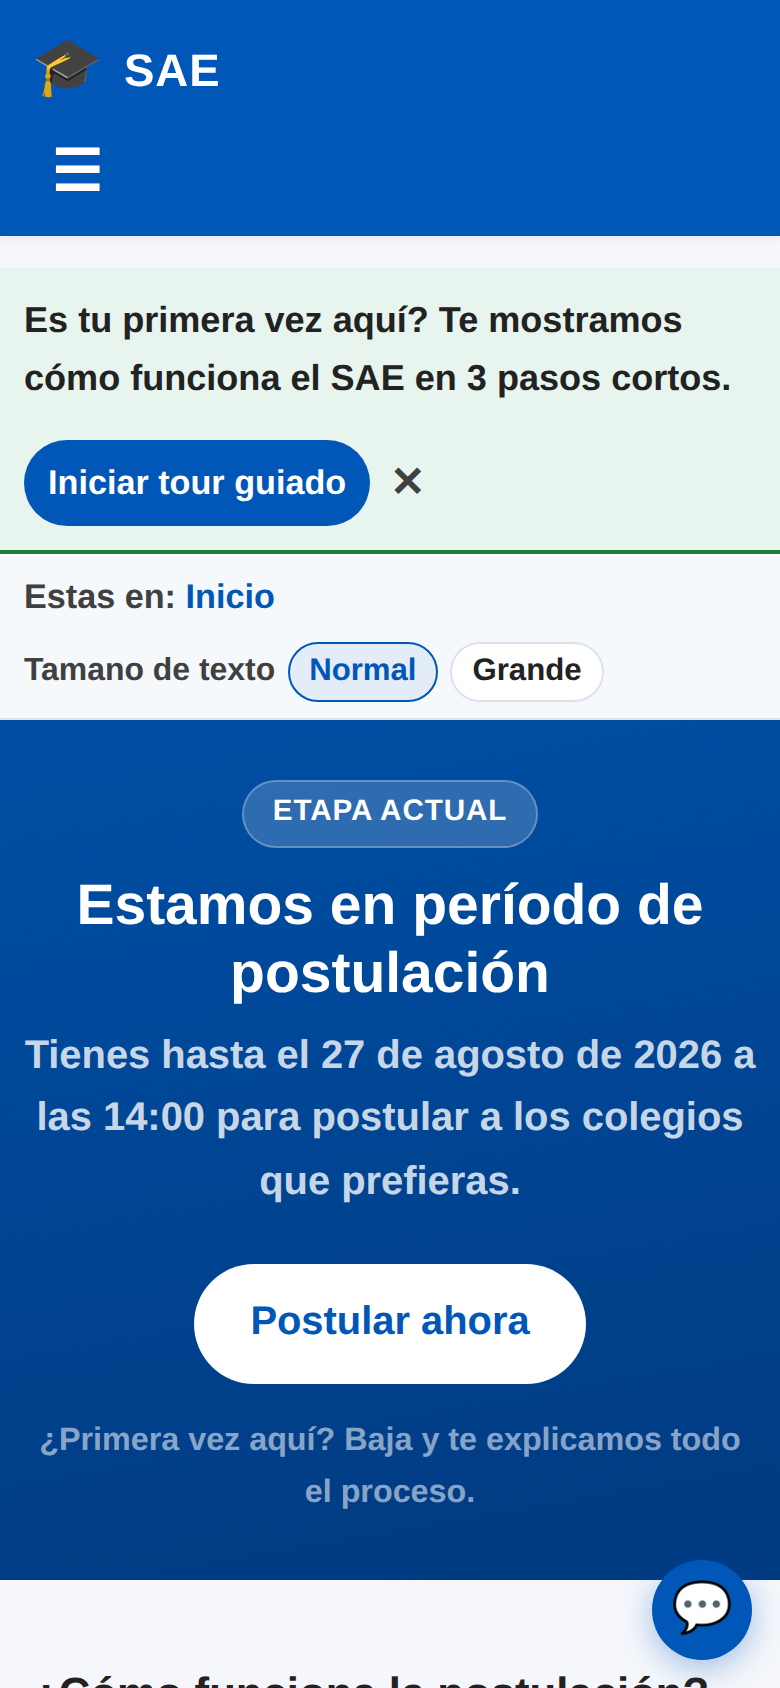
\includegraphics[width=\linewidth,height=0.6\textheight,keepaspectratio]{imagenes/propuesta/inicio.png}
\end{minipage}\hfill
\begin{minipage}[t]{0.44\textwidth}\centering
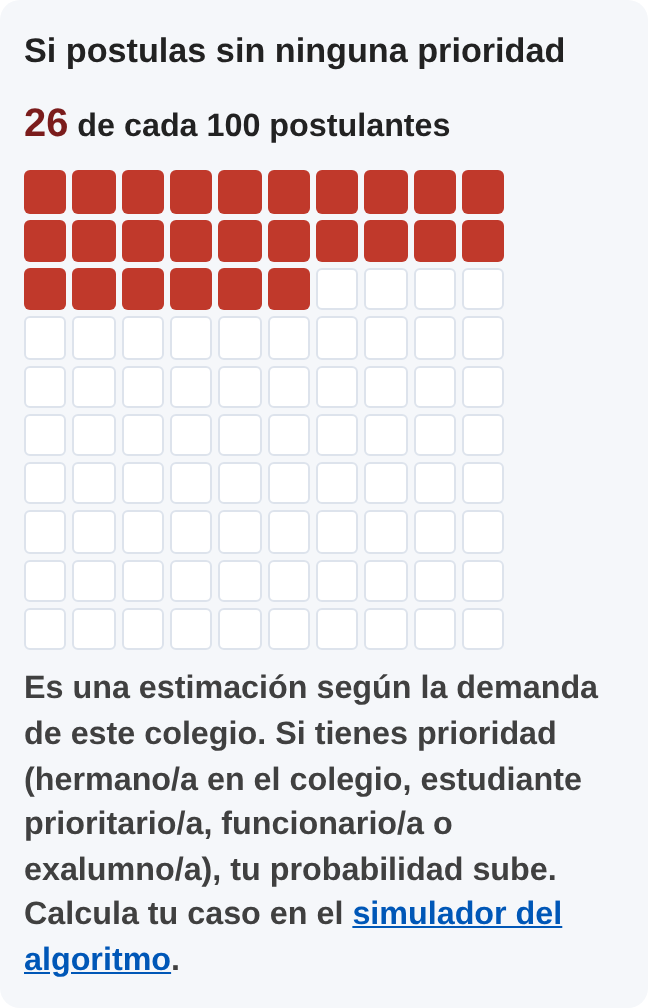
\includegraphics[width=\linewidth,height=0.6\textheight,keepaspectratio]{imagenes/propuesta/ficha-probabilidad.png}
\end{minipage}
\caption{Inicio con la etapa actual del proceso (izquierda) y estimación de probabilidad en formato de frecuencia en la ficha del Colegio San Martín (derecha).}
\label{fig:prop-inicio}
\end{figure}

\textbf{Cómo funciona el algoritmo y el proceso paso a paso.} La sección ``¿Cómo funciona?'' (Figura~\ref{fig:prop-algoritmo}, izquierda) explica en pasos cortos cómo se asigna un establecimiento: la familia arma su lista, el sistema aplica las prioridades que fija la ley y, cuando hay más postulantes que cupos, un sorteo por establecimiento. Primero entrega lo esencial y deja el detalle para quien lo busca, según el principio de divulgación progresiva. Incluye un simulador en que la persona elige establecimientos y prioridades y ve el resultado, y una reproducción paso a paso de cómo el sistema recorre su lista, aplicando el principio de controles interactivos con retroalimentación. Es la respuesta directa a la brecha más severa del diagnóstico: el 0\,\% de cumplimiento en \emph{transparencia y apertura}, que se explica porque no existe ninguna sección que explique el algoritmo. La vista ``El proceso paso a paso'' (Figura~\ref{fig:prop-algoritmo}, derecha) ordena las cinco etapas oficiales ---postulación, asignación, resultados, período complementario y matrícula---, destaca cinco reglas de alto impacto antes de empezar e incluye el calendario del proceso de admisión 2027.

\begin{figure}[htbp]
\centering
\begin{minipage}[t]{0.44\textwidth}\centering
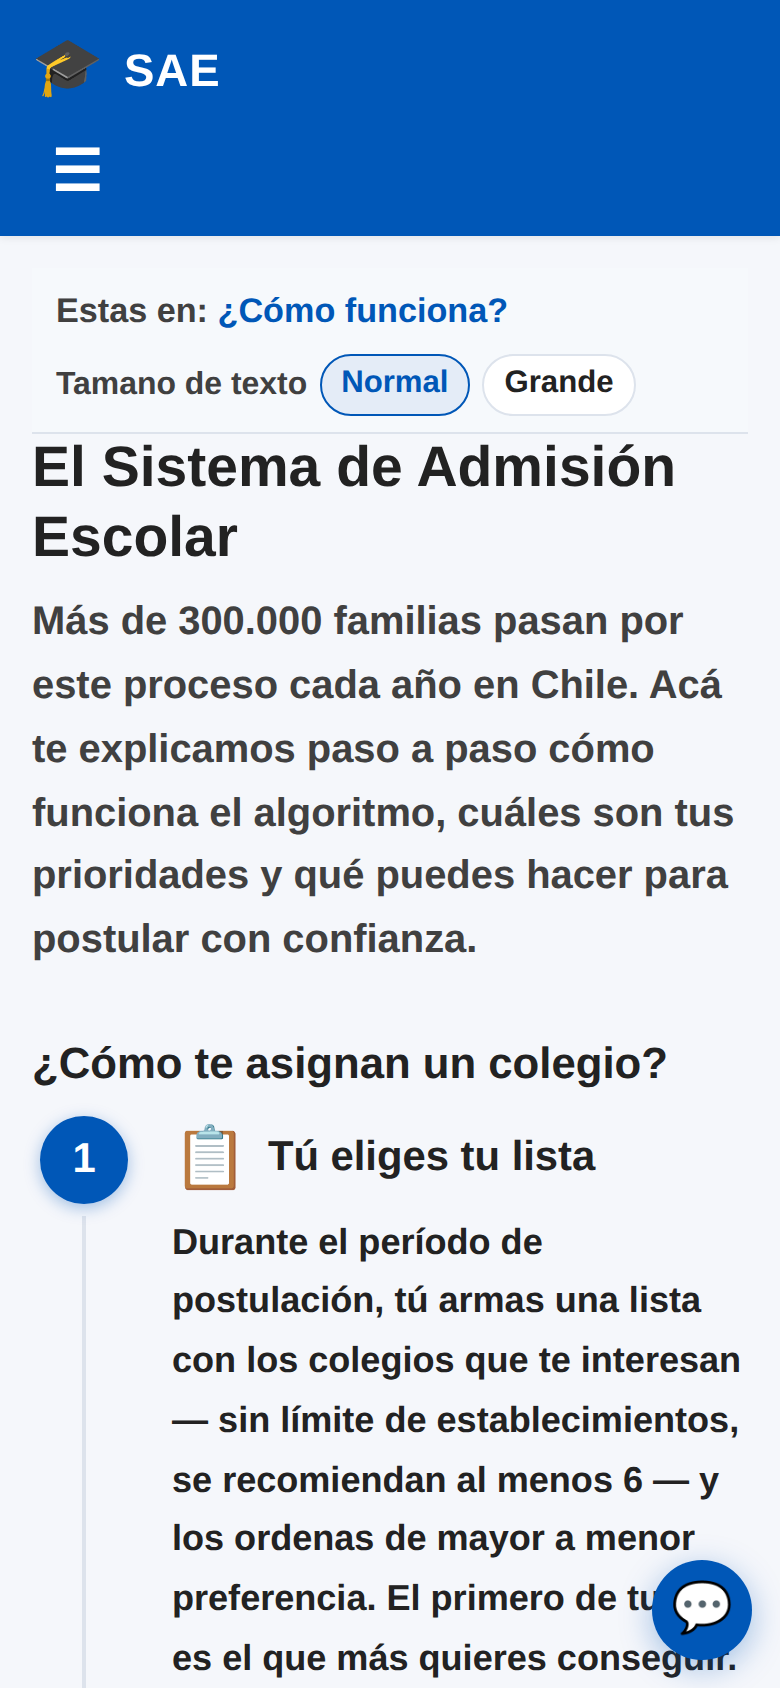
\includegraphics[width=\linewidth,height=0.6\textheight,keepaspectratio]{imagenes/propuesta/algoritmo.png}
\end{minipage}\hfill
\begin{minipage}[t]{0.44\textwidth}\centering
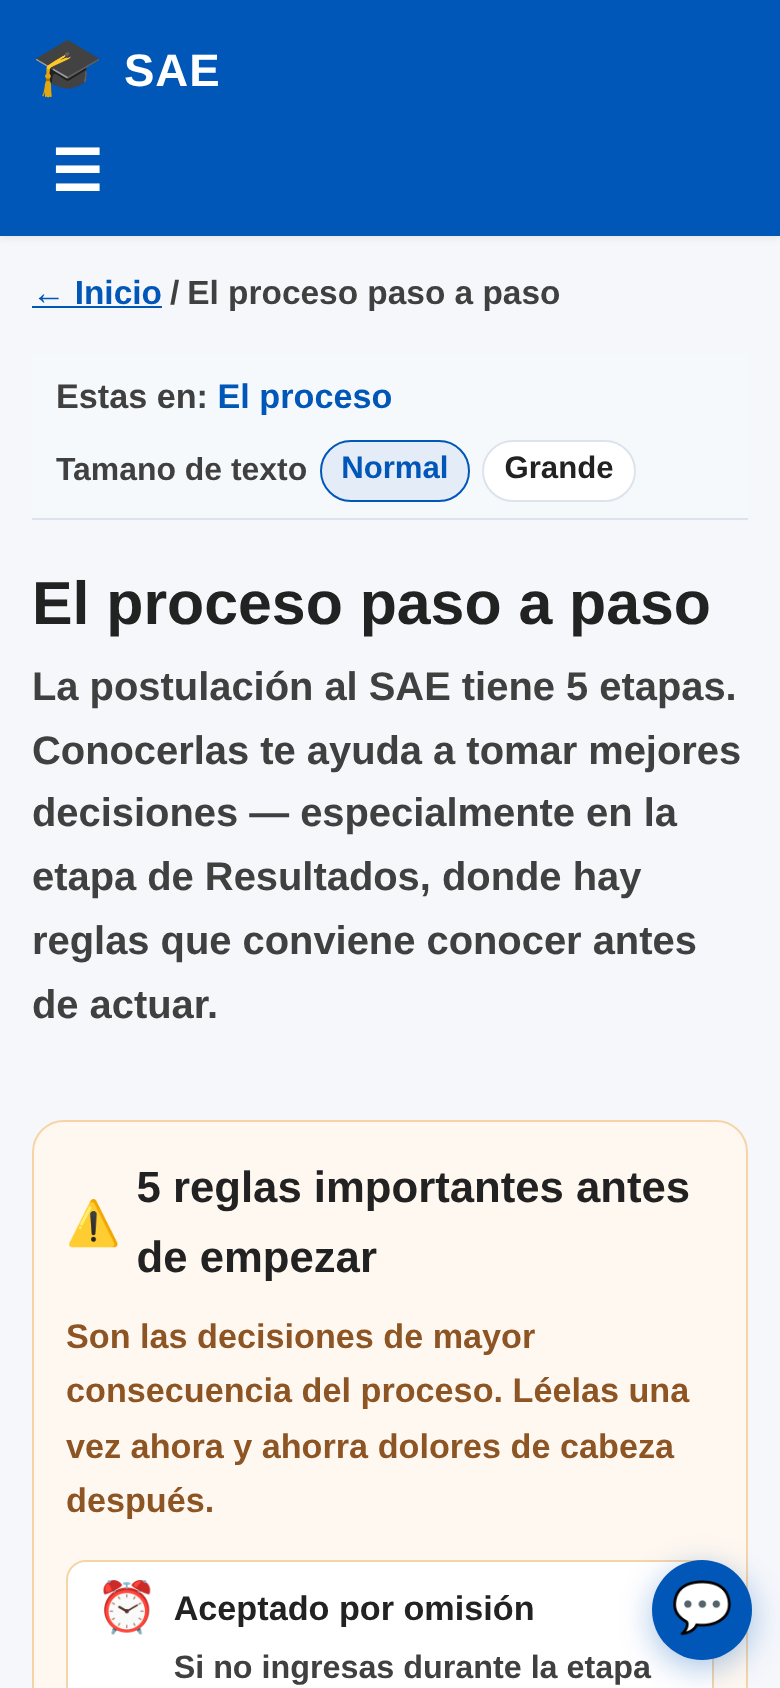
\includegraphics[width=\linewidth,height=0.6\textheight,keepaspectratio]{imagenes/propuesta/proceso.png}
\end{minipage}
\caption{Explicación del algoritmo de asignación (izquierda) y vista de las cinco etapas del proceso (derecha).}
\label{fig:prop-algoritmo}
\end{figure}

\section{El flujo de postulación}\label{sec:prop-postular}

El flujo de postulación es el caso de estudio central de la validación. Reproduce los datos, las declaraciones y las reglas del SAE real ---documentados a partir del sitio oficial y del video instructivo del Ministerio de Educación---, y agrega sobre ellos la capa de explicación que el sistema real no tiene.

\subsection{Paso 1: identificarse}

Tras ingresar con ClaveÚnica, la familia ve a sus hijos e hijas registrados en el Estado, con el curso que cursa hoy cada uno, su establecimiento actual y el curso al que entraría si postula (Figura~\ref{fig:prop-paso1}, izquierda). Nadie viene marcado: la familia elige a quién postular. Si marca a más de uno, la pantalla explica la postulación familiar en bloque, y a quien no se marca le explica que sigue en su establecimiento y no pierde su matrícula. Después, los datos de la estudiante y el domicilio aparecen ya cargados, para que la familia los \textbf{verifique} en lugar de escribirlos, con una opción para corregirlos, y se declara ser su apoderado o apoderada legal (Figura~\ref{fig:prop-paso1}, derecha). La precarga desde ClaveÚnica aborda la brecha de \emph{interoperabilidad}: en la plataforma real la cuenta de apoderado se crea por separado, pese a que ClaveÚnica ya contiene esos datos.

\begin{figure}[htbp]
\centering
\begin{minipage}[t]{0.44\textwidth}\centering
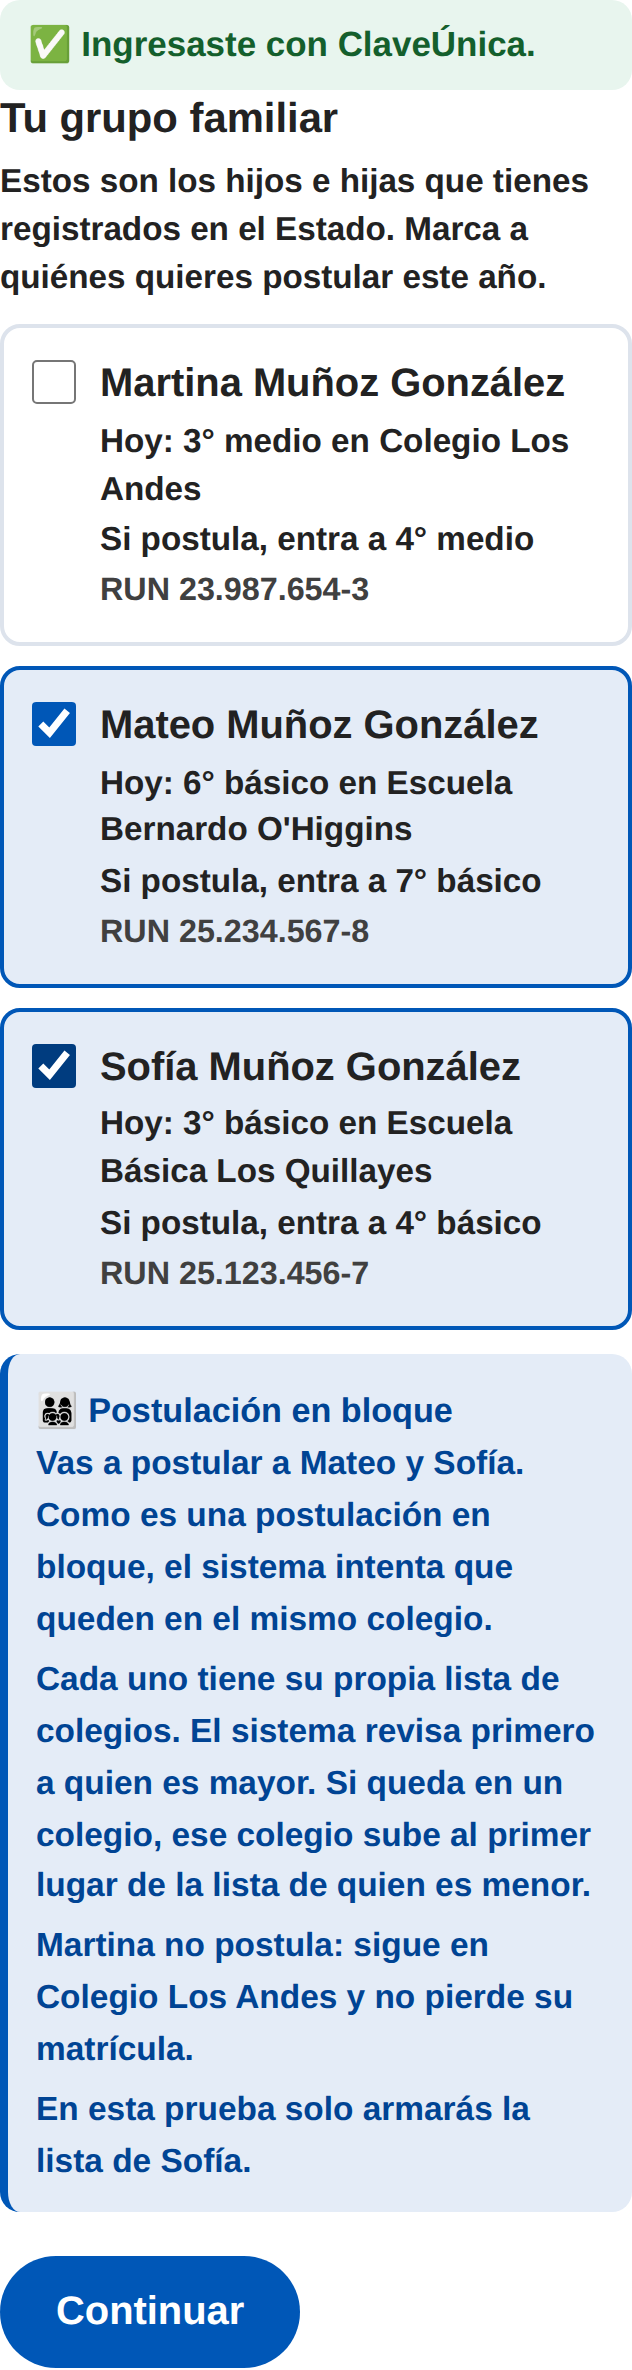
\includegraphics[width=\linewidth,height=0.6\textheight,keepaspectratio]{imagenes/propuesta/A-paso1-grupo-familiar.png}
\end{minipage}\hfill
\begin{minipage}[t]{0.44\textwidth}\centering
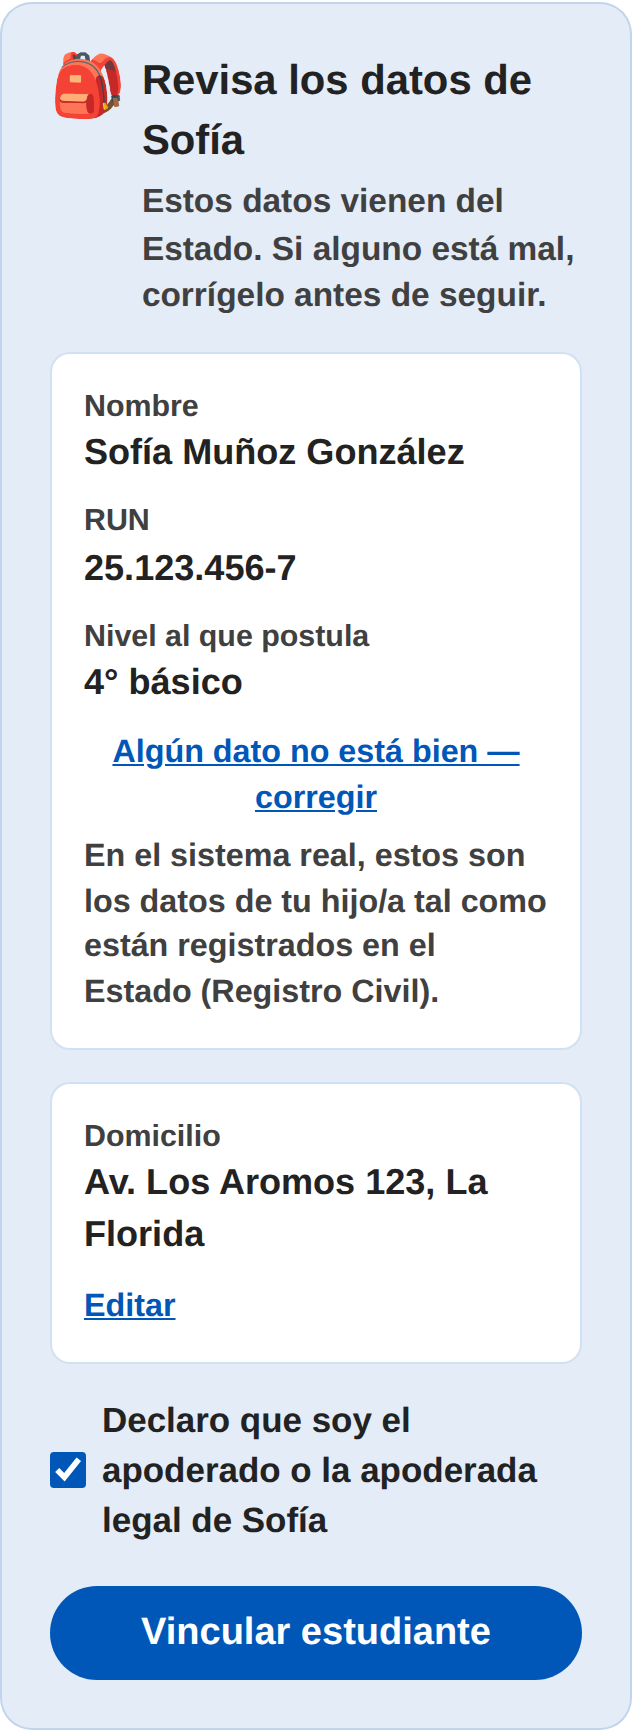
\includegraphics[width=\linewidth,height=0.6\textheight,keepaspectratio]{imagenes/propuesta/A-paso1-verificacion.png}
\end{minipage}
\caption{Paso~1: elección de quiénes postulan dentro del grupo familiar (izquierda) y verificación de los datos precargados, con la declaración de apoderada (derecha).}
\label{fig:prop-paso1}
\end{figure}

\subsection{Paso 2: armar y ordenar la lista}

El paso~2 separa el catálogo de establecimientos disponibles (Figura~\ref{fig:prop-paso2}, izquierda) de la lista propia, ordenada por preferencia (Figura~\ref{fig:prop-paso2}, derecha). Como en el SAE real, no hay tope de establecimientos y la región funciona como filtro, no como restricción. En la lista, cada establecimiento muestra su número de preferencia, su demanda, sus vacantes y la probabilidad estimada de obtener un cupo ---26 de cada 100 en el Colegio San Martín, donde la familia no tiene ningún vínculo, y 99 de cada 100 en el Colegio Los Andes, donde estudia una hermana---. Debajo, un recuadro indica la prioridad que la familia tiene \textbf{en ese establecimiento}: hermano o hermana, hijo o hija de funcionario y exalumno o exalumna son prioridades que valen solo en el colegio correspondiente. Esta es una explicación contextualizada a la situación de la familia y no una descripción general del sistema. La lista se reordena con botones o arrastrando, y un lector de pantalla anuncia cada cambio.

\begin{figure}[htbp]
\centering
\begin{minipage}[t]{0.44\textwidth}\centering
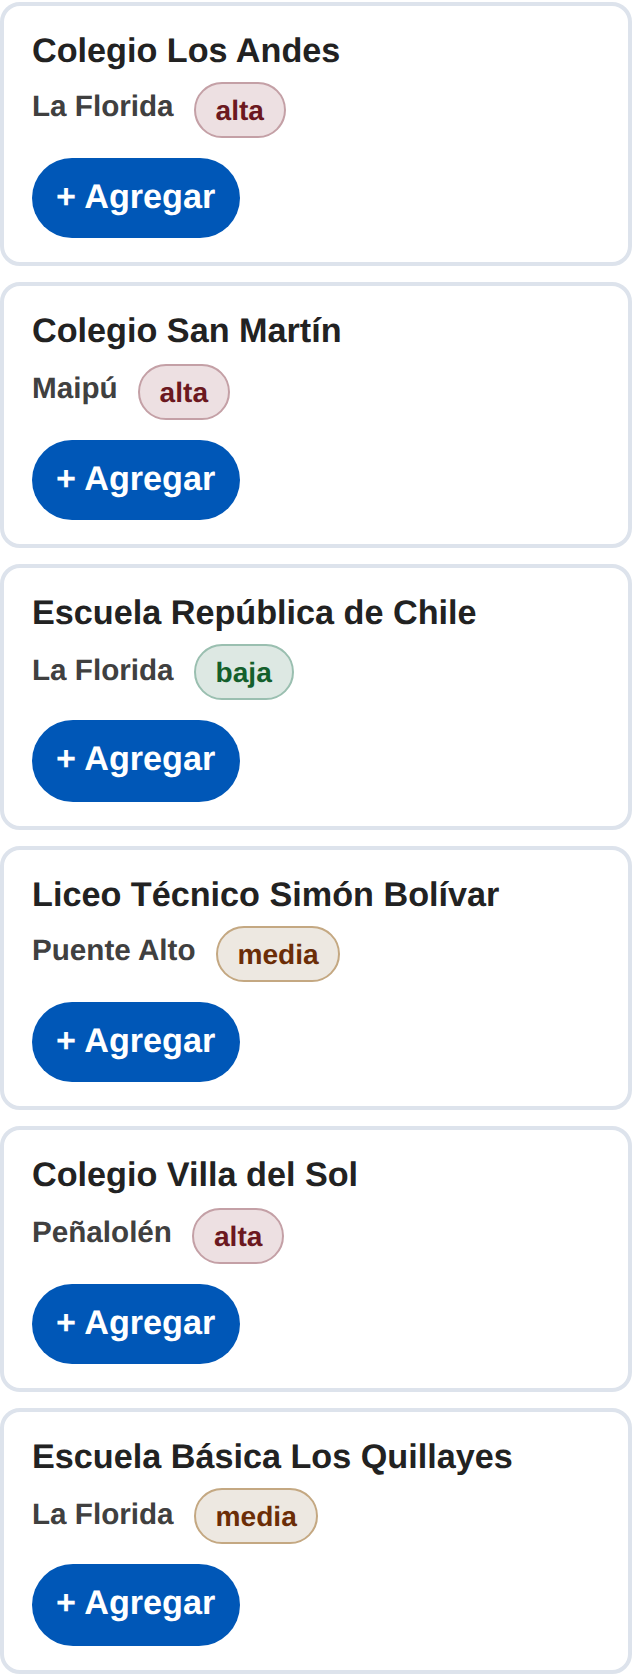
\includegraphics[width=\linewidth,height=0.6\textheight,keepaspectratio]{imagenes/propuesta/A-paso2-catalogo.png}
\end{minipage}\hfill
\begin{minipage}[t]{0.44\textwidth}\centering
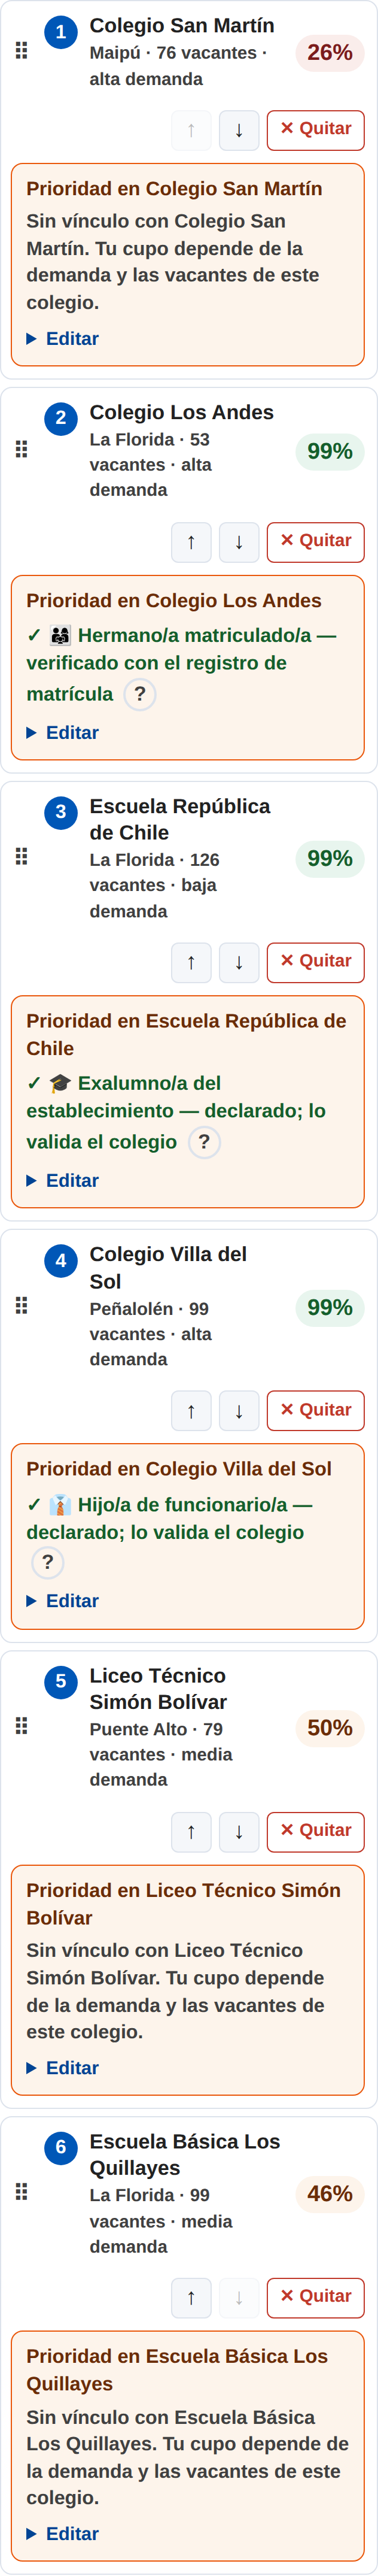
\includegraphics[width=\linewidth,height=0.6\textheight,keepaspectratio]{imagenes/propuesta/A-paso2-tu-lista.png}
\end{minipage}
\caption{Paso~2: catálogo de establecimientos (izquierda) y lista propia con la probabilidad estimada y la prioridad de la familia en cada establecimiento (derecha).}
\label{fig:prop-paso2}
\end{figure}

La decisión de diseño más directamente ligada a la pregunta de investigación está en el recuadro ``¿Qué hace el orden de tu lista?'' (Figura~\ref{fig:prop-paso3}, izquierda). Aborda el \emph{falso riesgo estratégico}: la creencia de que poner primero el establecimiento más deseado perjudica a la familia. El recuadro explica que cambiar el orden no cambia la probabilidad en cada establecimiento, sino solo en cuál de sus preferencias podría quedar, y por eso conviene poner primero el que más se quiere, en coherencia con la propiedad de \emph{strategy-proofness} de la Aceptación Diferida (Sección~\ref{sec:fase3-caso}). También aclara que se trata de una simulación con datos del año anterior y no del resultado, que el sistema calcula meses después.

\subsection{Paso 3: revisar y enviar}

El paso~3 resume la postulación completa antes de enviarla, con un enlace para editar cada sección, la postulación en bloque con el hermano y la fecha límite del proceso (Figura~\ref{fig:prop-paso3}, derecha). La aceptación de la jornada y del proyecto educativo de los establecimientos, que el SAE real exige, se pide una sola vez al enviar, para toda la lista. Al confirmar, la familia puede descargar un comprobante.

\begin{figure}[htbp]
\centering
\begin{minipage}[t]{0.44\textwidth}\centering
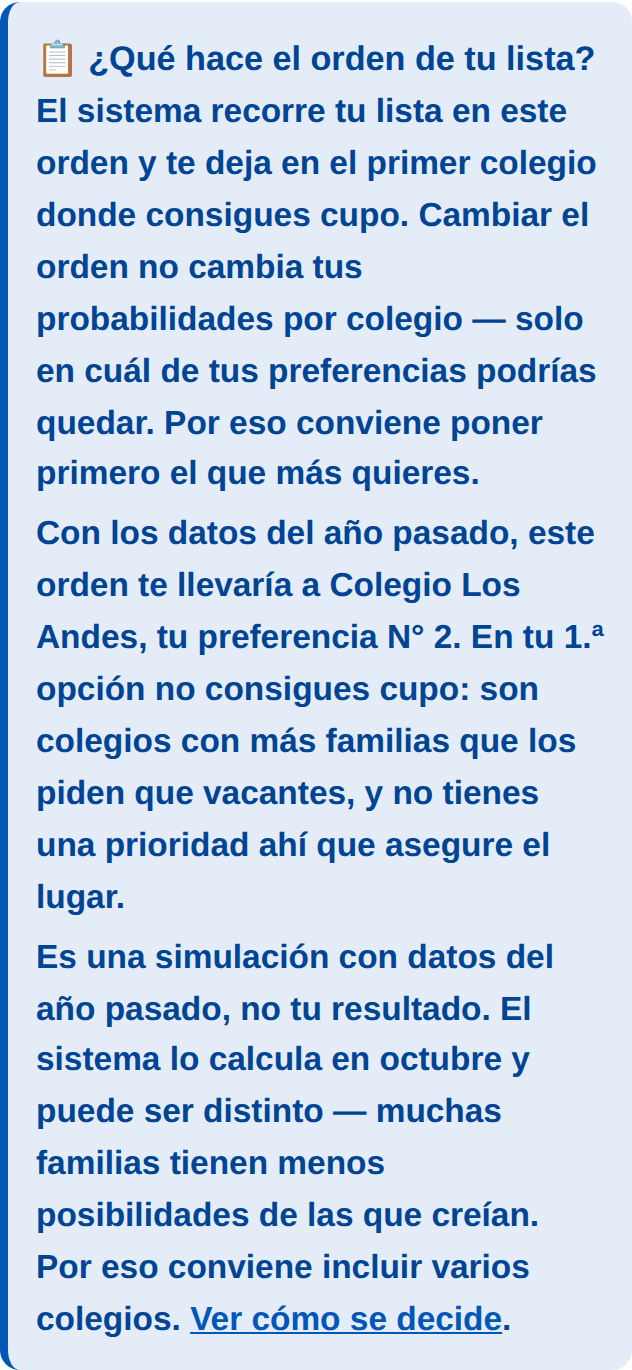
\includegraphics[width=\linewidth,height=0.6\textheight,keepaspectratio]{imagenes/propuesta/A-paso2-orden-lista.png}
\end{minipage}\hfill
\begin{minipage}[t]{0.44\textwidth}\centering
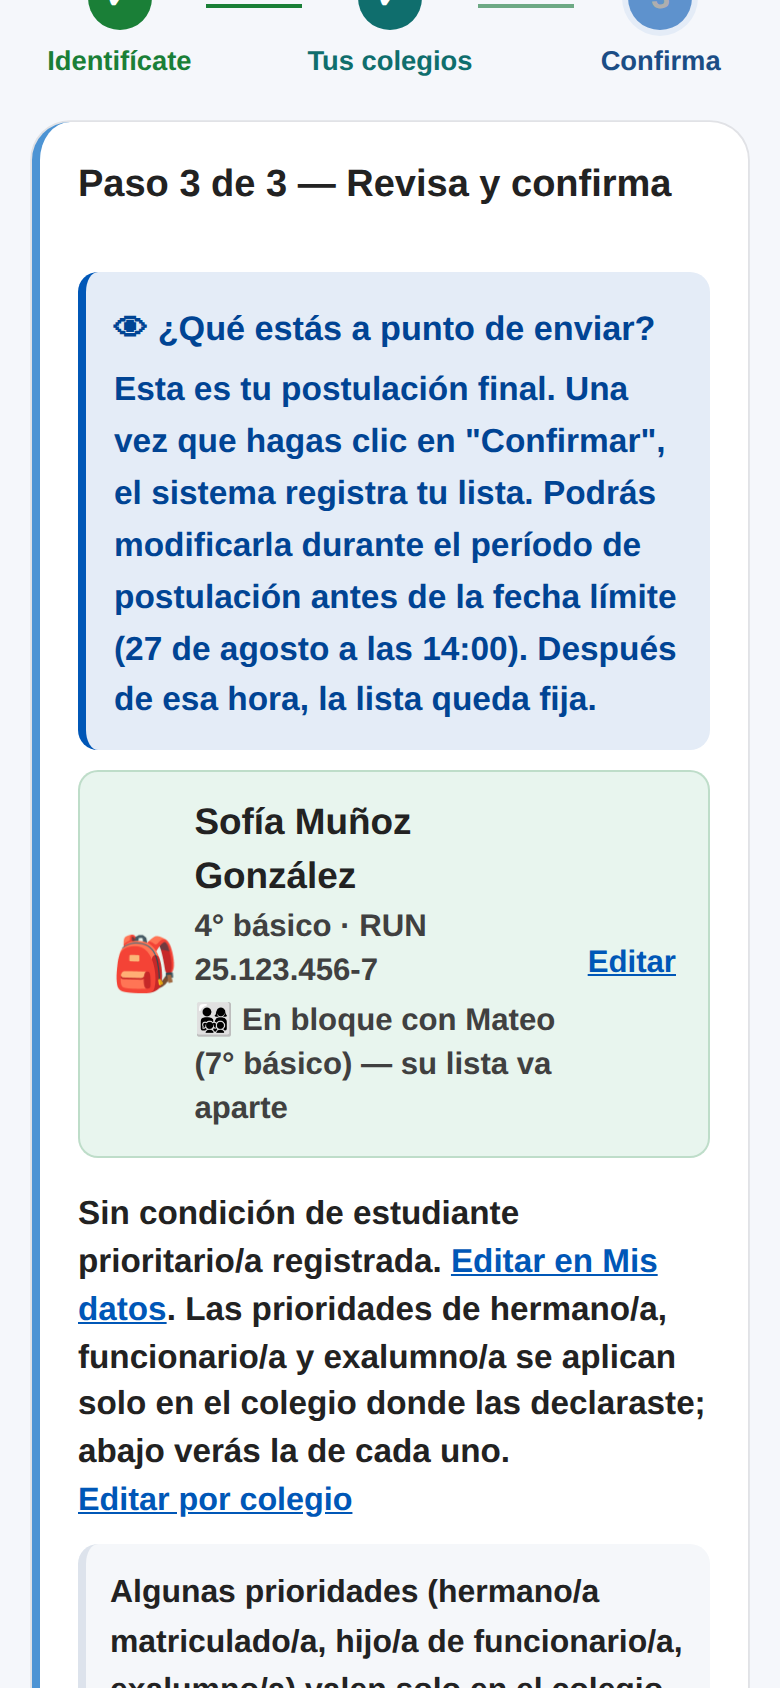
\includegraphics[width=\linewidth,height=0.6\textheight,keepaspectratio]{imagenes/propuesta/A-paso3-revision.png}
\end{minipage}
\caption{Explicación de qué hace el orden de la lista, al final del paso~2 (izquierda), y revisión de la postulación en el paso~3 (derecha).}
\label{fig:prop-paso3}
\end{figure}

\section{El resultado y su explicación}\label{sec:prop-resultado}

Para que el estudio comparativo pueda observar la reacción al resultado dentro de la misma sesión, el prototipo lo adelanta; en el proceso real se conoce meses después. La tarjeta de resultado indica el establecimiento asignado y en qué preferencia quedó (Figura~\ref{fig:prop-resultado}, izquierda). En el caso de estudio, la familia no queda en su primera preferencia, el Colegio San Martín, y queda en la segunda, el Colegio Los Andes.

Debajo, la sección ``¿Por qué te asignaron este colegio?'' (Figura~\ref{fig:prop-resultado}, derecha) explica ese resultado específico: una tabla compara la situación de la familia en el establecimiento que no obtuvo ---sin vínculo, demanda alta--- con la del que obtuvo ---prioridad por hermana---, y una explicación desplegable detalla que en el Colegio San Martín hubo más familias que cupos, que la familia no tenía ahí ninguna prioridad y que el sorteo de ese establecimiento vale solo para él y no afectó sus otras opciones. Es la aplicación más directa del principio de explicabilidad contextualizada, y su redacción sigue los marcos de diseño: atribuir el resultado a reglas y no a un juicio sobre la familia, usar lenguaje de proceso en lugar de describir al sistema como si decidiera, y cerrar recordando que el sistema no puede crear cupos ni asegurar la primera preferencia.

\begin{figure}[htbp]
\centering
\begin{minipage}[t]{0.44\textwidth}\centering
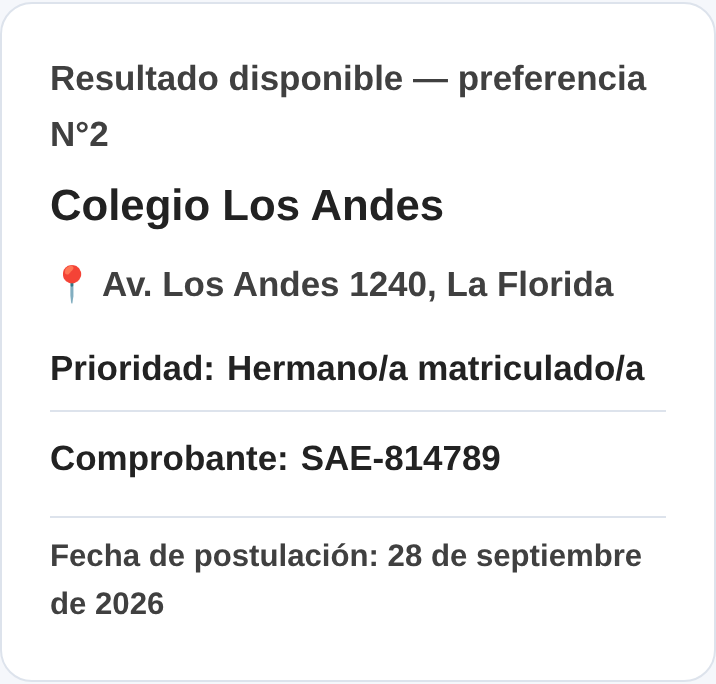
\includegraphics[width=\linewidth,height=0.6\textheight,keepaspectratio]{imagenes/propuesta/A-resultado.png}
\end{minipage}\hfill
\begin{minipage}[t]{0.44\textwidth}\centering
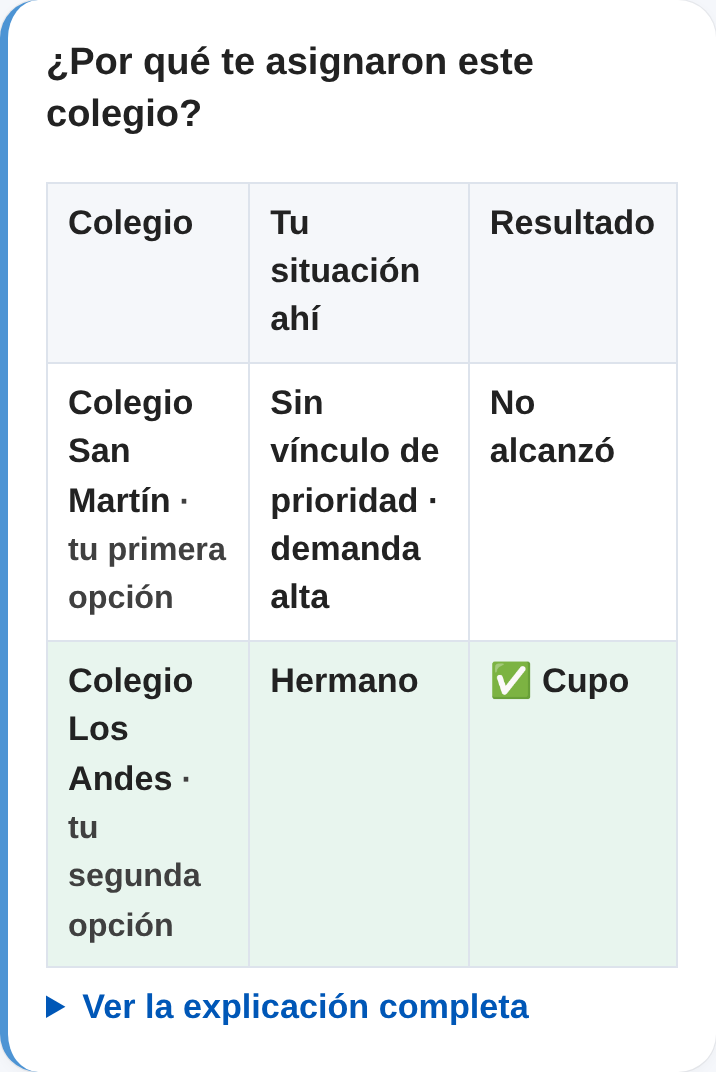
\includegraphics[width=\linewidth,height=0.6\textheight,keepaspectratio]{imagenes/propuesta/A-resultado-explicacion.png}
\end{minipage}
\caption{Resultado de la postulación (izquierda) y explicación de por qué se asignó ese establecimiento (derecha).}
\label{fig:prop-resultado}
\end{figure}

\section{La condición de control}\label{sec:prop-control}

El estudio comparativo necesita una versión del prototipo sin la capa de explicación, que funcione como aproximación al SAE real. En lugar de construir una segunda aplicación, el mismo prototipo tiene un modo de control que el moderador activa al inicio de cada sesión. En ese modo se ocultan la sección que explica el algoritmo, las probabilidades estimadas, el recuadro sobre el orden de la lista y la explicación del resultado; se conservan los elementos que son fidelidad al sistema real, como la precarga de datos, la prioridad de la familia en cada establecimiento y las declaraciones. La Figura~\ref{fig:prop-control} muestra las mismas dos pantallas que en la condición completa: la lista sin probabilidades (compárese con la Figura~\ref{fig:prop-paso2}) y el resultado sin su explicación (compárese con la Figura~\ref{fig:prop-resultado}). Como la lógica de asignación es la misma, el establecimiento asignado es idéntico en ambas condiciones.

\begin{figure}[htbp]
\centering
\begin{minipage}[t]{0.44\textwidth}\centering
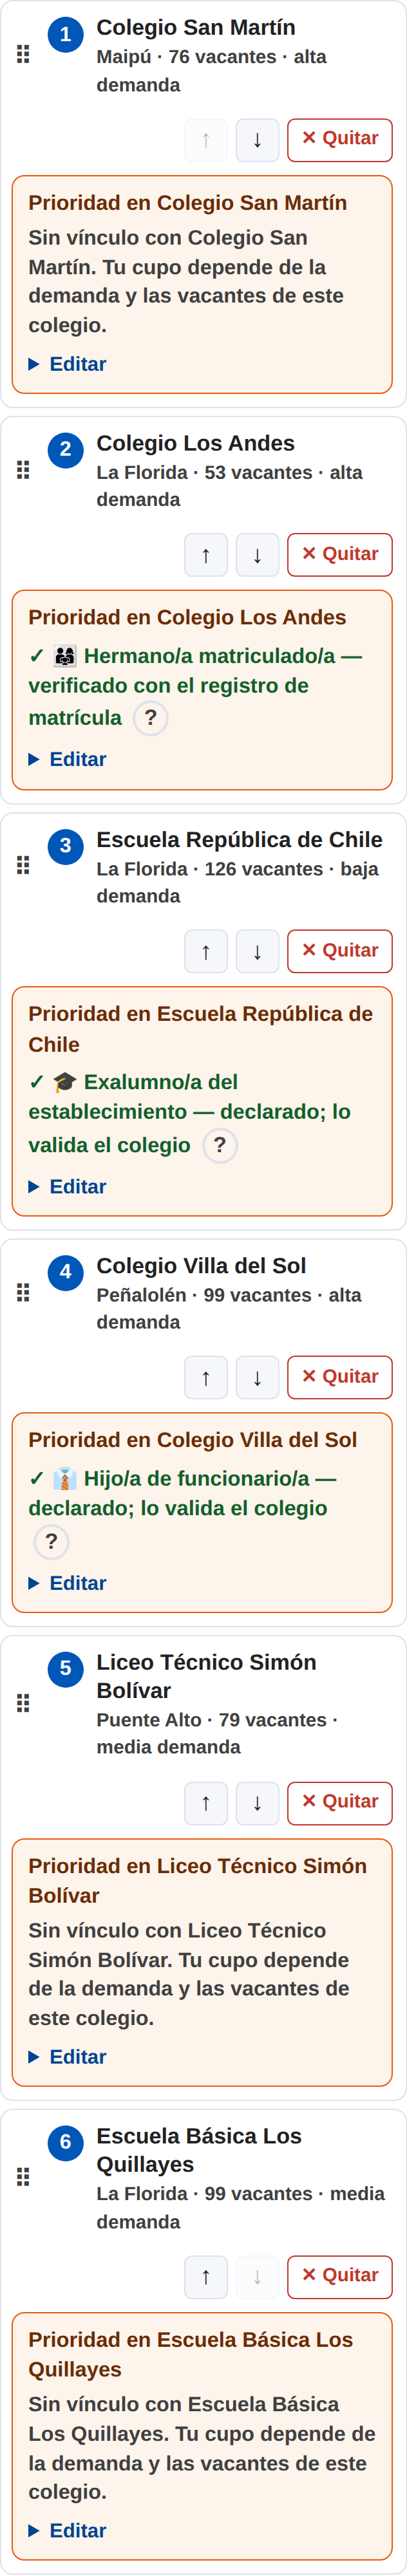
\includegraphics[width=\linewidth,height=0.6\textheight,keepaspectratio]{imagenes/propuesta/B-paso2-tu-lista.png}
\end{minipage}\hfill
\begin{minipage}[t]{0.44\textwidth}\centering
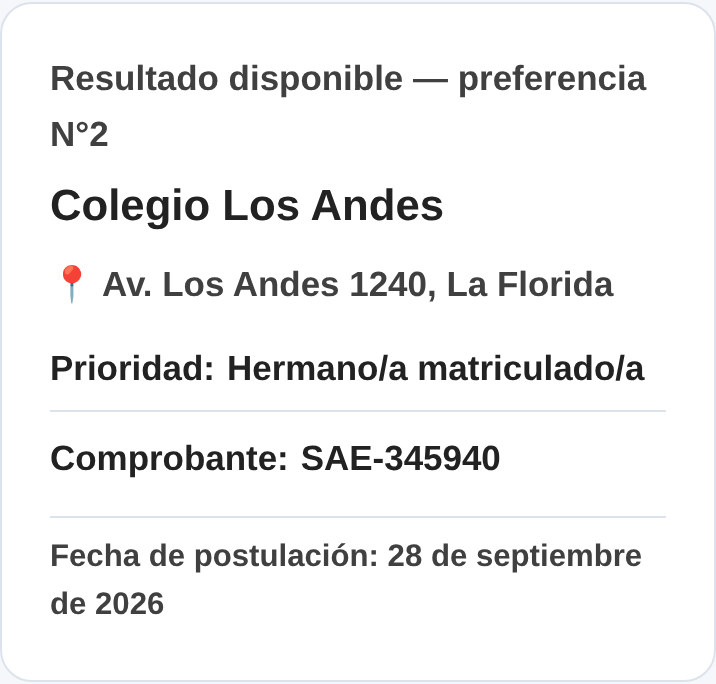
\includegraphics[width=\linewidth,height=0.6\textheight,keepaspectratio]{imagenes/propuesta/B-resultado.png}
\end{minipage}
\caption{Condición de control: la lista sin probabilidades (izquierda) y el resultado sin explicación (derecha).}
\label{fig:prop-control}
\end{figure}

\section{Síntesis: brechas y principios}\label{sec:prop-sintesis}

La Tabla~\ref{tab:prop-sintesis} resume qué elemento de la propuesta aborda cada brecha del diagnóstico y con qué principio. La brecha de \emph{audiovisualidad} no se aborda: el prototipo no incorpora videos ni infografías animadas, lo que queda como trabajo futuro.

\begin{table}[htbp]
\centering
\caption{Elementos de la propuesta, brecha del diagnóstico que abordan y principio de diseño que aplican.}
\label{tab:prop-sintesis}
\small
\begin{tabular}{p{4.2cm}p{3.6cm}p{5.2cm}}
\toprule
\textbf{Elemento} & \textbf{Brecha} & \textbf{Principio} \\
\midrule
Explicación del algoritmo, simulador y reproducción paso a paso & Transparencia y apertura & Divulgación progresiva; controles interactivos con retroalimentación \\
Probabilidad por establecimiento en formato ``X de cada 100'' & Transparencia y apertura & Presentación multidimensional; comunicación de riesgo \\
Explicación de qué hace el orden de la lista & Transparencia y apertura & Gestión de expectativas; \emph{strategy-proofness} \\
Explicación del resultado & Transparencia y apertura & Explicabilidad contextualizada \\
Buscador, orden de la vitrina y ficha & Búsqueda y encontrabilidad & Presentación multidimensional \\
Precarga de datos desde ClaveÚnica & Interoperabilidad & Fidelidad al SAE real: la familia verifica los datos en lugar de escribirlos \\
Lenguaje claro, letra aumentada y alto contraste & Legibilidad e inclusión & Accesibilidad web \\
\bottomrule
\end{tabular}
\end{table}
